\chapter{Appendix 1 - Wyniki testu sposobów komunikacji radiowej}

\begin{table}[H]
	\caption {Wartości zmierzone dla eksperymentu nr 1, w którym Router TP-Link TD-W8970 był transmiterem sygnału Wifi}
\begin{center}
		\begin{tabular}{|c|c|}
			\hline
			Wartość (dBm) & Ilość pomiarów \\ 
			\hline
			-44 & 1\\
			\hline
			-43 & 6\\
			\hline
			-42 & 5\\
			\hline
			-41 & 11\\
			\hline
			-40 & 28\\
			\hline
			-39 & 38\\
			\hline
			-38 & 38\\
			\hline
			-37 & 33\\
			\hline
			-36 & 3\\
			\hline
		\end{tabular}
\end{center}
\end{table}
\begin{figure}[H]			
	\centering
	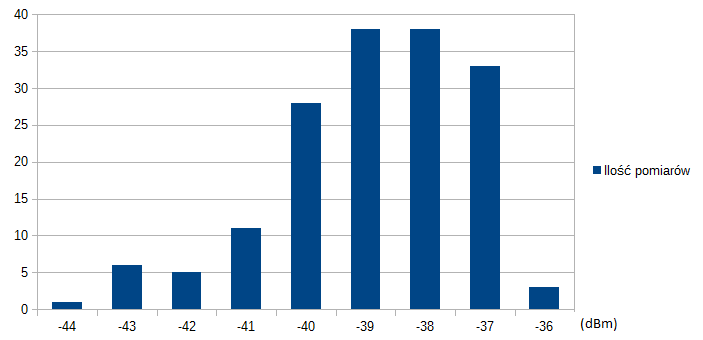
\includegraphics[width=1.0\textwidth]{wykres_wifi_1}
\end{figure}
\begin{table}[H]
	\caption{Wartości zmierzone dla eksperymentu nr 1, w którym Samsung Grand 2 był  transmiterem Bluetooth}
\begin{center}
		\begin{tabular}{|c|c|}
			\hline
			Wartość (dBm) & Ilość pomiarów \\ 
			\hline
			-64 & 1\\
			\hline
			-62 & 4\\
			\hline
			-61 & 10\\
			\hline
			-60 & 14\\
			\hline
			-59 & 9\\
			\hline
			-58 & 13\\
			\hline
			-57 & 11\\
			\hline
			-56 & 27\\
			\hline
			-55 & 15\\
			\hline
			-54 & 9\\
			\hline
		\end{tabular}
\end{center}
\end{table}
\begin{figure}[H]			
\centering
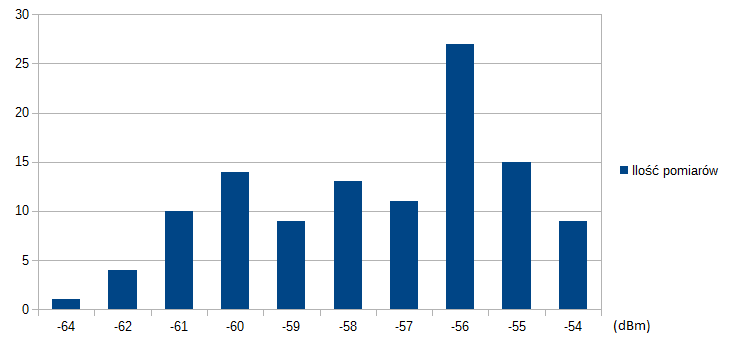
\includegraphics[width=1.0\textwidth]{wykres_bluetooth_1}
\end{figure}
\begin{table}[H]
	\caption {Wartość siły sygnałów Wifi, dla których przeszkodą była książka przy dystansie 1 metra} 
\begin{center}
	\begin{tabular}{|c|c|}
		\hline
		Wartość (dBm) & Ilość pomiarów \\ 
		\hline
		-44 & 3\\
		\hline
		-43 & 15\\
		\hline
		-42 & 21\\
		\hline
		-41 & 57\\
		\hline
		-40 & 78\\
		\hline
		-39 & 8\\
		\hline
	\end{tabular}
\end{center}
\end{table}
\begin{figure}[H]			
\centering
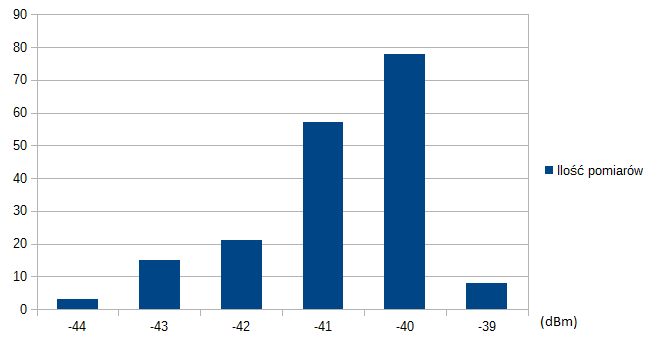
\includegraphics[width=1.0\textwidth]{wykres_wifi_2}
\end{figure}
\begin{table}[H]
	\caption {Wartość siły sygnałów Bluetooth, dla których przeszkodą była książka przy dystansie 1 metra}
\begin{center}
		\begin{tabular}{|c|c|}
			\hline
			Wartość (dBm) & Ilość pomiarów \\ 
			\hline
			-68 & 1\\
			\hline
			-67 & 3\\
			\hline
			-66 & 2\\
			\hline
			-65 & 7\\
			\hline
			-64 & 1\\
			\hline
			-63 & 4\\
			\hline
			-62 & 12\\
			\hline
			-61 & 12\\
			\hline
			-60 & 11\\
			\hline
			-59 & 10\\
			\hline
			-58 & 5\\
			\hline
			-57 & 2\\
			\hline
		\end{tabular}
\end{center}
\end{table}
\begin{figure}[H]			
\centering
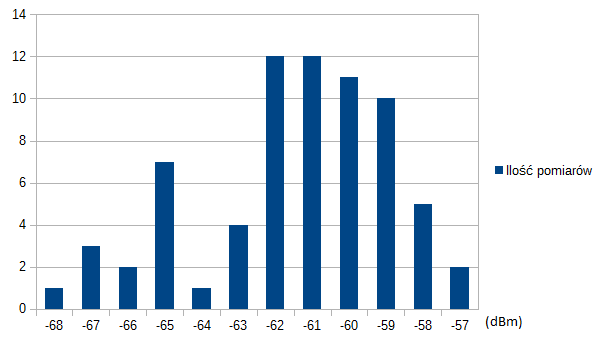
\includegraphics[width=1.0\textwidth]{wykres_bluetooth_2}
\end{figure}
\begin{table}[H]
	\caption {Wartość siły sygnałów Wifi, dla których przeszkodą były drzwi przy dystansie 2 metrów}
\begin{center}
		\begin{tabular}{|c|c|}
			\hline
			Wartość (dBm) & Ilość pomiarów \\ 
			\hline
			-57 & 1\\
			\hline
			-55 & 1\\
			\hline
			-51 & 1\\
			\hline
			-48 & 98\\
			\hline
			-45 & 2\\
			\hline
		\end{tabular}
\end{center}
\end{table}
\begin{figure}[H]			
\centering
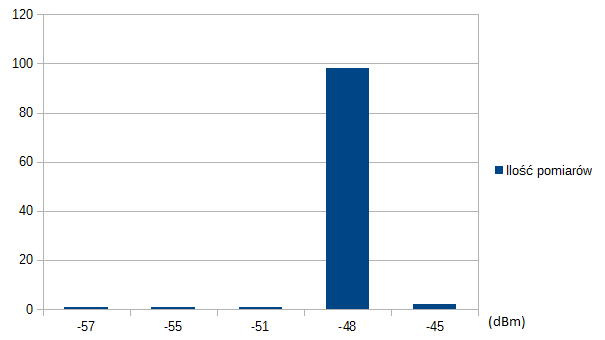
\includegraphics[width=1.0\textwidth]{wykres_wifi_3}
\end{figure}
\begin{table}[H]
	\caption {Wartość siły sygnałów Bluetooth, dla których przeszkodą były drzwi przy dystansie 2 metrów}
\begin{center}
		\begin{tabular}{|c|c|}
			\hline
			Wartość (dBm) & Ilość pomiarów \\ 
			\hline
			-104 & 1\\
			\hline
			-80 & 1\\
			\hline
			-79 & 1\\
			\hline
			-76 & 1\\
			\hline
			-73 & 1\\
			\hline
			-72 & 3\\
			\hline
			-71 & 5\\
			\hline
			-70 & 4\\
			\hline
			-69 & 8\\
			\hline
			-68 & 12\\
			\hline
			-67 & 17\\
			\hline
			-66 & 15\\
			\hline
			-65 & 9\\
			\hline
			-64 & 8\\
			\hline
			-63 & 13\\
			\hline
			-62 & 4\\
			\hline
			-61 & 4\\
			\hline
		\end{tabular}
\end{center}
\end{table}
\begin{figure}[H]			
\centering
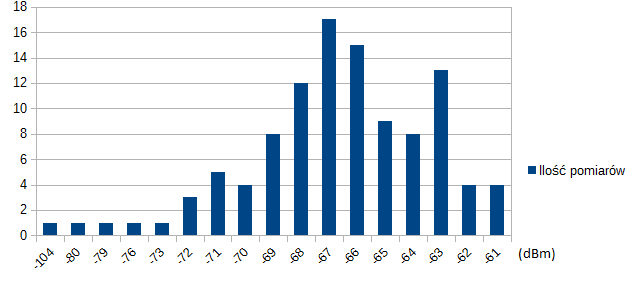
\includegraphics[width=1.0\textwidth]{wykres_bluetooth_3}
\end{figure}
\begin{table}[H]
	\caption {Wartość siły sygnałów Wifi, dla których przeszkodą była ściana przy dystansie 2 metrów}
\begin{center}
		\begin{tabular}{|c|c|}
			\hline
			Wartość (dBm) & Ilość pomiarów \\ 
			\hline
			-57 & 3\\
			\hline
			-56 & 9\\
			\hline
			-55 & 3\\
			\hline
			-54 & 3\\
			\hline
			-51 & 3\\
			\hline
			-50 & 25\\
			\hline
			-49 & 18\\
			\hline
			-48 & 18\\
			\hline
			-47 & 8\\
			\hline
			-46 & 7\\
			\hline
			-45 & 3\\
			\hline
			-37 & 3\\
			\hline
			-35 & 9\\
			\hline
		\end{tabular}
\end{center}
\end{table}
\begin{figure}[H]			
\centering
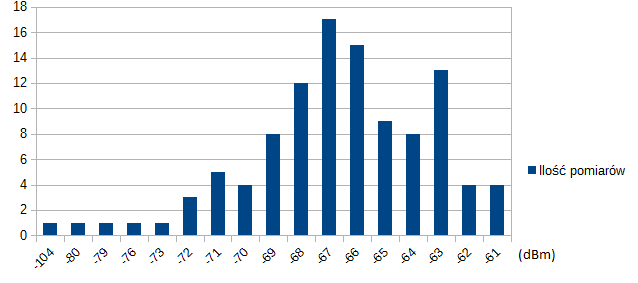
\includegraphics[width=1.0\textwidth]{wykres_wifi_4}
\end{figure}
\begin{table}[H]
	\caption {Wartość siły sygnałów Bluetooth, dla których przeszkodą była ściana przy dystansie 2 metrów}
\begin{center}
	\begin{tabular}{|c|c|}
		\hline
		Wartość (dBm) & Ilość pomiarów \\ 
		\hline
		-99 & 2\\
		\hline
		-86 & 1\\
		\hline
		-84 & 1\\
		\hline
		-79 & 1\\
		\hline
		-78 & 2\\
		\hline
		-77 & 1\\
		\hline
		-76 & 1\\
		\hline
		-75 & 2\\
		\hline
		-74 & 7\\
		\hline
		-73 & 1\\
		\hline
		-72 & 2\\
		\hline
		-71 & 6\\
		\hline
		-70 & 7\\
		\hline
		-69 &11\\
		\hline
		-68 & 5\\
		\hline
		-67 & 5\\
		\hline
		-66 & 4\\
		\hline
		-65 & 8\\
		\hline
		-64 & 2\\
		\hline
		-63 & 6\\
		\hline
		-62 & 9\\
		\hline
		-61 & 7\\
		\hline
		-60 & 4\\
		\hline
		-59 & 5\\
		\hline
		-58 & 2\\
		\hline
		-57 & 3\\
		\hline
		-56 & 2\\
		\hline
		-55 & 3\\
		\hline
	\end{tabular}
\end{center}
\end{table}
\begin{figure}[H]			
\centering
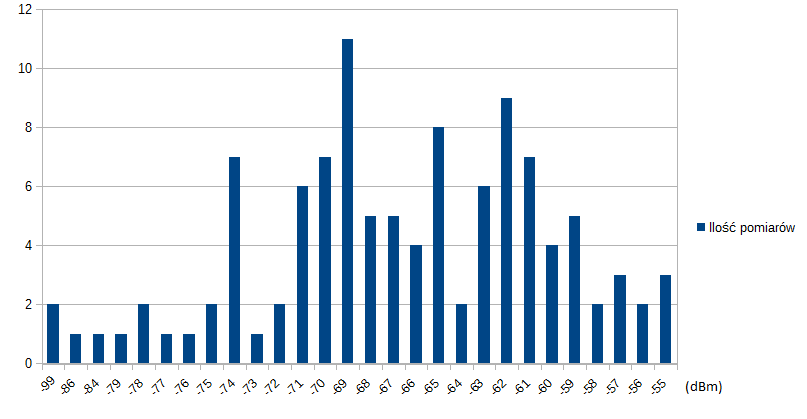
\includegraphics[width=1.0\textwidth]{wykres_bluetooth_4}
\end{figure}